\section{Grundlagen}
Im folgenden Kapitel werden die theoretischen Grundlagen behandelt, die für das Verständnis dieser Arbeit notwendig sind. Dabei geht es in erster Linie um allgemeine Begrifflichkeiten aus dem wirtschaftlichen Kontext des zu entwickelnen Programms.

\subsection{ERP-Systeme}
ERP ist ein Akronym für den englischen Begriff \glqq{}Enterprise Ressource Planning\grqq{}, also das Planen von Unternehmensressourcen, u.a. in den Bereichen Beschaffung, Produktion, Vertrieb, Personalwirtschaft und Finanzwesen. \footcite[Vgl.][523]{wibuch} Ein ERP-System beschreibt somit eine Software, die Prozesse aus diesen Bereichen in einem Anwendungspaket integriert und die dabei anfallenden Daten in einer zentralen Datenbank abspeichert. Dadurch werden Redundanzen in der Datenhaltung vermieden und die Umsetzung von bereichsübergreifenden Unternehmensprozessen ermöglicht \footcite[Vgl.][523]{wibuch}. ERP-Systeme nutzen in der Regel eine Client-Server-Architektur und sind komponentenorientiert, das heißt, Unternehmen können, je nach Anforderungen ihrer Wertschöpfungsprozesse, die benötigten Komponenten frei wählen. Dadurch ist eine schrittweise Einführung der ERP-Software, über einen längeren Zeitraum, möglich. \footcite[Vgl.][524 f.]{wibuch}

\subsection{SAP}
\subsubsection{Die SAP SE}
Die SAP SE wurde im Jahr 1972 von fünf ehemaligen IBM-Mitarbeitern unter dem Namen \glqq{}\underline{S}ystem\underline{a}nalyse und \underline{P}rogrammentwicklung GbR\grqq{}\footcite[Vgl.][]{think-ing}  mit dem Ziel gegründet, eine Standardanwendungssoftware für die Echtzeitverarbeitung zu entwickeln.  Im Jahr 1973 wurde durch die SAP mit dem \glqq{}System RF\grqq{} das erste Produkt für die Finanzbuchhaltung vorgestellt, was den Grundstein für die erste SAP-Generation \glqq{}SAP R/1\grqq{} legen sollte. Durch die ständigen Weiterentwicklungen wurde das System stets erweitert und fand bei immer mehr Kunden anklang. 1976 wurde die Gesellschaft bürgerlichen Rechts aufeglöst und in eine GmbH überführt. Im selben Jahr wurde bereits mit nur 25 Mitarbeitern ein Umsatz von 3,81 Mio. DM erzielt. \footcite[Vgl.][]{sap-fruehejahre}\\Im Jahr 1979 folgt schließlich die zweite Produktgeneration \glqq{}SAP R/2\grqq{}, die eine höhere Stabilität mit sich brachte und in weitere Geschäftsbereiche vordrang. In der Generation R/2 waren bereits die Module RF für Finanzbuchhaltung, RK für die Kostenrechnung, RM für Materialwirtschaft, Produktionsplanung und Instandhaltung, RP für die Personalwirtschaft und RV für den Vertrieb verfügbar.\footcite[Vgl.][]{bewerbungsratgeber}\\Im Jahr 1988 wurde die SAP GmbH schließlich in eine Aktiengesellschaft überführt und startete an der Börse Frankfurt sowie in Stuttgart. Im selben Jahr erwirtschaftetet SAP bereits einen Umsatz von 245 Mio. DM und hatte bereits 940 Mitarbeiter. Bereits zu diesem Zeitpunkt war die dritte Generation \glqq{}SAP R/3\grqq{} in Entwicklung, die schließlich im Jahr 1992 erschien und, in Gegensatz zu ihren Vorgängern, auf einer Client-Server-Architektur aufgebaut war. Das führte dazu, dass SAP immer erfolgreicher wurde und auch international immer weiter expandierte, sodass im Jahr 1997 schließlich 1,6 Mrd. DM  Umsatz erwirtschaftet wurden. 1995 begann SAP damit, seine Vertriebsaktivitäten im deutschen Mittelstand auszubauen, da zuvor die Hauptkundenzielgruppe nur größere Unternehmen waren. In den darauffolgenden Jahren startete die SAP zusammen mit Microsoft seine Internetstrategie und setzte mit \glqq{}mySAP.com\grqq{} vermehrt den Fokus auf E-Commerce und E-Business-Lösungen und seit dem Jahr 2007 auch auf Business Intelligence.\footcite[Vgl.]{sap-fruehejahre} Ab dem Jahr 2009 richtete sich die SAP verstärkt auf die Bereiche der Datenbanktechnologie und Cloud Computing aus, woraus schließlich im Jahr 2011 die Datenbanktechnologie \glqq{}SAP HANA\grqq{} enstand, die vorallem Geschwindigkeitsoptimierungen in der Datenverarbeitung mit sich brachte. 2015 wurde schließlich die vierte, heute noch aktuelle, SAP-Generation \glqq{}SAP S/4HANA\grqq{} vorgestellt, die vollständig auf SAP S/4HANA basiert und eine moderne Benutzeroberfläche mit sich bringt, mit der Anwendungen auch auf mobilen Endgeräten dargestellt werden können. Auch bietet die SAP mit S/4HANA erstmalig Cloud-Lösungen für ihre Kunden, was besonders auf kleine und mittelständische Unternehmen abzielt.\footcite[Vgl.][]{sap-historie}\\ Im Jahr 2020 belief sich der Gesamtumsatz der SAP SE auf 27,338 Mrd. EUR, worauf alleine ca. 15 Mrd. EUR auf den Vertrieb von \glqq{}On-Premise\grqq{} Softwarelizenzen und -Support zurückzuführen sind und ca. weitere 8 Mrd. EUR auf die Umsätze mit Softwarelizenzen und -Support aus den Cloud-Plattformen zurückgehen. Nach Abzug der operativen Aufwendungen und der Steuern blieben davon 5,238 Mrd. EUR Gewinn.\footcite[Vgl.][S. 142]{sap2020-report} 

\begin{figure}[h]
    \centering
    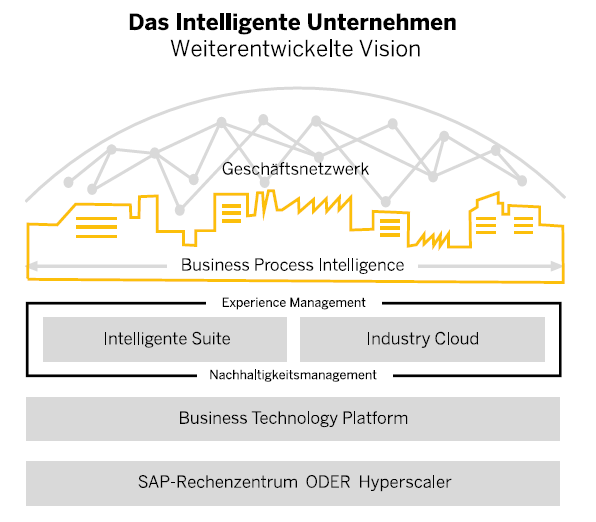
\includegraphics[scale=1]{Bilder/SAPIntelligentesUnternehmen.png}
    \caption[]{Das Intelligente Unternehmen (\cite[][S. 53]{sap2020-report})}
\end{figure}

Die SAP verfolgt derzeit die Vision ihre Kunden zu einem intelligenten Unternehmen zu entwickeln, in denen die Prinzipien der Innovation, Integration, Agilität und Geschwindigkeit an vorderster Stelle stehen. Außerdem alle Elemente eines Unternehmens verbunden werden und ineinandergreifen. Die Komponenten eines solchen intelligenten Unternehmens sind nach Vorstellungen der SAP ein Geschäftsnetzwerk, das die unternehmensübegreifenden Prozesse miteinander verknüpft, eine Business Process Intelligence, die die Geschäftsprozesse analysiert und optimiert, das Experience Management, das die Daten der Anwender, Kunden und Mitarbeiter analysiert, eine Business Technology Platform, die das Fundament für die Integration und Erweiterung von Anwendungen liefert und dem Kunden Möglichkeiten für künstliche Intelligenz, maschinelles Lernen und Prozessautomatisierung bietet, und einem SAP-Rechenzentrum oder einem Hyperscaler, also einem Infrastrucute-as-a-Service Anbieter wie Amazons AWS oder Microsoft Azure.\footcite[Vgl.][S. 53 f.]{sap2020-report}


\subsubsection{SAP-ERP}

\subsubsection{S/4HANA} 

\subsubsection{SAP HANA}

\subsection{Transformation}
\subsubsection{Definition}
Unter einer Transformation versteht man im allgemeinen einen grundlegenden Wandel, der durch bestimmte Faktoren, wie z.B. einer sprunghafte wirtschaftlichen, oder technologischen Entwicklung hervorgerufen wird. Die Transformation hält dabei idR. über einen längeren Zeitraum an und ist erst beendet, sobald sich die neu geschaffenen Strukturen etabliert und gefestigt haben.\footcite[Vgl.][]{difu}\\ Im betriebswirtschaftlichen Kontext versteht man unter einer Transformation (oder auch Business Transformation) die gezielte Umgestaltung eines Unternehmens und seiner Geschäftsprozesse, um auf veränderte Bedingungen am Markt einzugehen und sich ihnen anzupassen. Dabei ist das Ziel durch effizientere und vereinfachte Geschäftsprozesse einen Mehrwert in Form von niedrigeren Kosten bei gleichbleibender, oder bestenfalls verbesserter Qualität zu erreichen und dabei zusätzlich die Kundenzufriedenheit zu steigern.\footcite[Vgl.][]{leanix}

\subsubsection{Die vier R der Transformation}
In den 1990er-Jahren wurde durch Gouillart und Kelly das Modell der \glqq{}Vier R der Transformation\grqq{} \footcite[Vgl.][]{4r-modell} entwickelt, was eine mögliche Form der Business Transformation darstellen soll. Aus diesem Modell hat die Beratungsgesellschaft Gemini Consulting (später in der Capgemini SE aufgegangen)\footcite[Vgl.][]{gemini-died} ein Produkt entwickelt, indem die vier R für vier verschiedene Transformationsdimensionen stehen:\\
\begin{figure}[h]
    \centering
    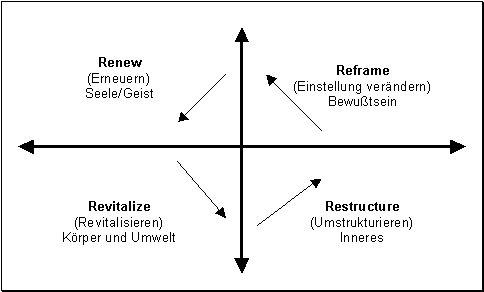
\includegraphics[scale=0.5]{Bilder/businesstransformationManagementportal.png}
    \caption[]{Die vier R der Transformation}
\end{figure}
\begin{itemize}
    \item[] \emph{Reframing (dt. Einstellungsveränderung)} soll in einem Unternehmen dazu beitragen die Sichtweise auf sich selbst zu überdenken um sich dadurch von alten Denkmustern zu befreien. Um diese Einstellungsveränderung anzustoßen ist es wichtig, dass die Mitarbeiter motiviert werden und davon überzeugt sind durch die eingesetze Energie einen Mehrwert zu generieren. Im nächsten Schritt muss anschließend eine Vision definiert werden, die sich erheblich von der präsenten Realität absetzt um im Anschluss daraus Ziele und Messgrößen zu entwickeln. 
    \item[] \emph{Restructuring (dt. Restrukturierung)} 
    \item[] \emph{Revitalising (dt. Wiederbelebung)}
    \item[] \emph{Renewing (dt. Erneuerung)}
\end{itemize}

\subsubsection{Digitale Transformation}
-- Digitale Transformation
\subsubsection{Besonderheiten der S/4HANA Transformation}
